\subsection{Gridded Components}

Gridded Components encapsulate the computational data and the
grid on which it is located.  A Gridded Component contains
the following object hierarchy:

\scalebox{0.70}{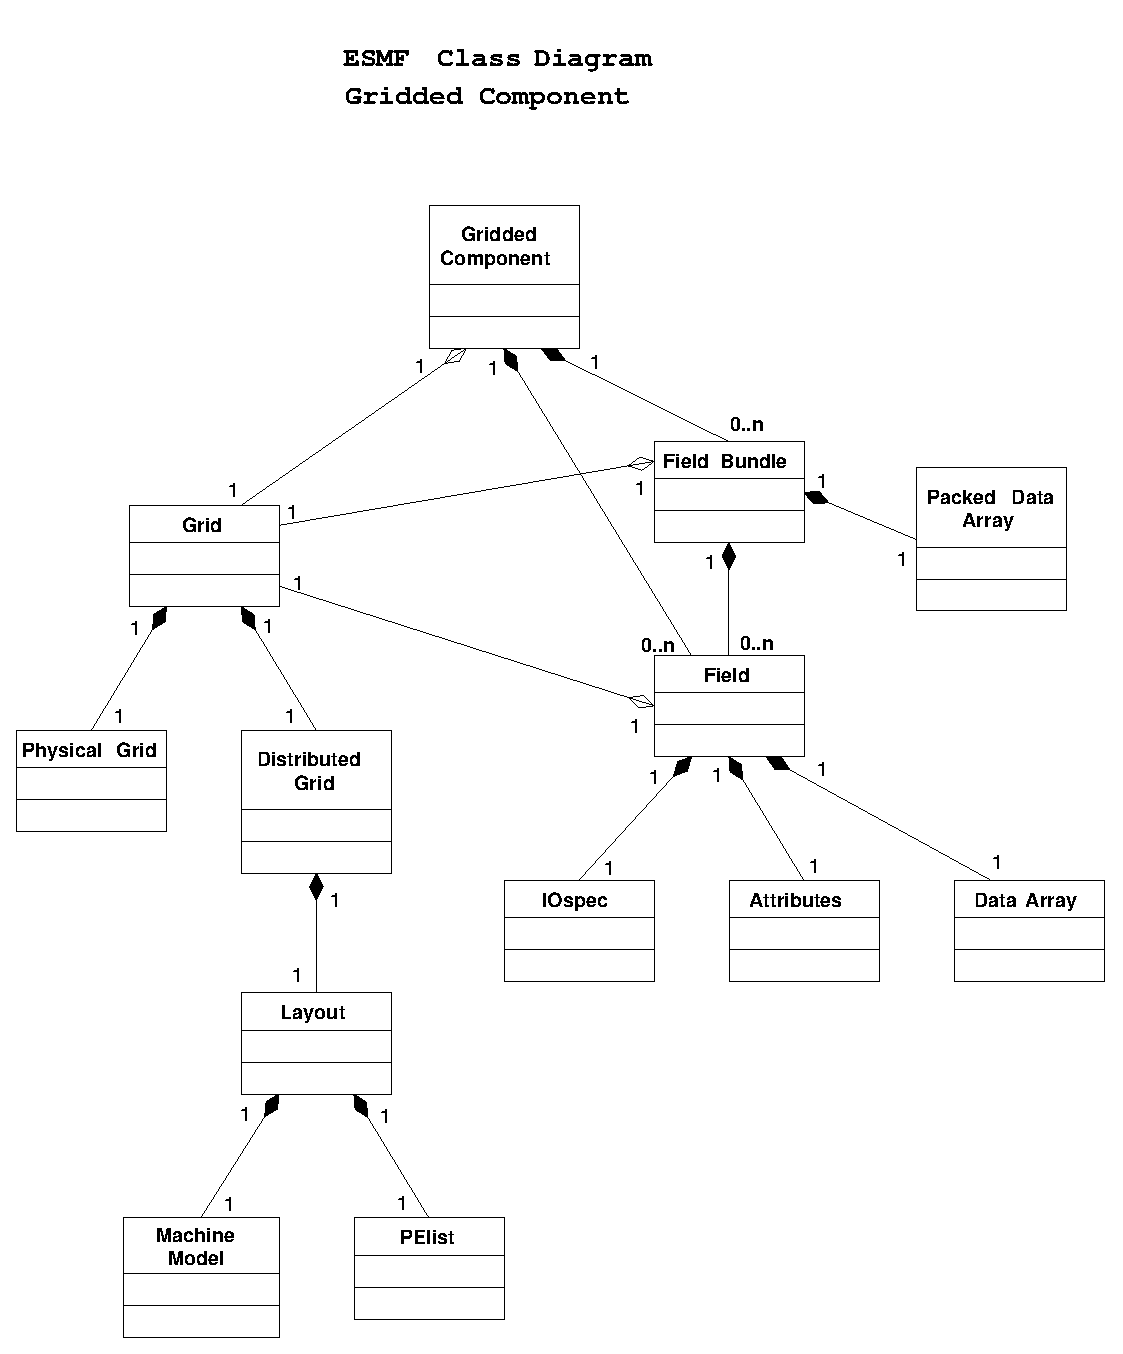
\includegraphics{ESMF_DataStructureHierarchy.eps}}


\subsubsection{Bundle (ESMF\_Bundle)}
\label{sec:bundle} 
\begin{description}
\item [Description] A Bundle contains one or more Fields which are defined on the
same Grid.  It allows the application to manipulate multiple fields in an identical
manner with a single set of calls.  It also allows the option of interleaving data
from multiple fields into a Packed Data Array (see Section~\ref{packeddataarray}) for
more efficient memory access patterns.
\item [Function] The Bundle class is an aggregation of the Field class.  It provides methods 
for getting and setting fields.  It provides methods for querying information about the
underlying grid.  It provides methods for requesting the packing of data, the
reordering of that packed data, and detaching and attaching the data.
\end{description}

\subsubsection{Packed Data Array (ESMF\_PackedData)}
\label{sec:packeddataarray} 
\begin{description}
\item [Description] A Packed Data Array contains data from one or more Fields, where the
data items are interleaved in memory. The application may use a packed array to maintain
locality of reference while iterating the array, or for ease in subsetting multiple
data values in one operation.
\item [Function] The PackedData class provides methods for packing and querying arrays,
subsetting the data, and repacking the data in a different order.  The PackedData object
contains an Ordering object to maintain the information about the structure of the packing.
It is contained by a Bundle object.  Application access is through Bundle methods.
\end{description}

\subsubsection{Field (ESMF\_Field)}
\label{sec:field} 
\begin{description} 
\item [Description] A Field represents a single physical field or the components of a 
vector field.  It is the basic data carrying object in the system.  It includes both
the data and the grid on which the data is defined.  The main application interfaces
for accessing data are here.
\item [Function] The Field object is a composition of the Data Array object, an optional
Mask object, an optional IOspec object, and it aggregates a Grid object.  It provides
methods for getting, setting, and querying the data array, the grid, the mask and
the I/O spec.  It provides methods for detaching and attaching data from the field.
While data is detached it is the responsibility of the application.  A Field object
provides methods for subsetting, regridding, and reordering memory layout of data.
\end{description}

\subsubsection{Mask (ESMF\_Mask)}
\label{sec:mask} 
\begin{description}
\item [Description] A Mask describes a subset of data items, for example to indicate
the valid values which represent ocean points (and not land) in an ocean model.  
It may be specified at the Grid object level, but it is stored below the Field level 
for effiency of computation.
\item [Function] The Mask class is an optional part of a Field class.  It provides methods
for getting and setting valid values.
\end{description}

\subsubsection{Data Array (ESMF\_Data)}
\label{sec:dataarray} 
\begin{description}
\item [Description] A Data Array is a list of data values plus information about
the data itself.
\item [Function] The Data class contains the data as well as information about the data,
including the data type (e.g. float,
integer), the machine type (e.g. IEEE float, Cray float), data count, data dimensionality
(e.g. scalar, vector).  It provides methods for querying all information about the data,
returning a pointer to the memory location of the start of the data, and conversion routines
for altering the characteristics of the data.  Information about how the data array is laid
out in memory is contained in an Ordering class.
\end{description}

\subsubsection{Ordering (ESMF\_Ordering)}
\label{sec:ordering} 
\begin{description}
\item [Description] A Ordering is the description of how multidimentional data have been
linearized in memory.  This includes both multidimensional array index information (e.g. C-order
vs Fortran-order) as well as vector or tensor data item information (e.g. all Xs then all
Ys vs [X,Y], [X,Y] tuples).
\item [Function] An Ordering object is associated with a single Data object.  It provides
methods to query the current memory organization and methods to reorder the Data object.
\end{description}

\subsubsection{Grid (ESMF\_Grid)}
\label{sec:ordering} 
\begin{description}
\item [Description] A Grid is the general representation of the coordinate information for
the computation.  It contains both the logical presenatation of the grid as well as the
decomposition of the grid into subgrids for processing in parallel on a
multiprocessor system.
\item [Function] The Grid class is the composition of a PhysGrid and a DistGrid object.  
It is aggregated into the Field and the Bundle objects.  It provides methods to the
Field and Bundle classes for obtaining coordinate, indexing, and decomposition information.
\end{description}

\subsubsection{Physical Grid (ESMF\_PhysGrid)}
\label{sec:physgrid} 
\begin{description}
\item [Description] A Physical Grid is a discrete representation of a continuous physical space.
There are a multitude of types of physical grids.
The grid contains the physical coordinates, usually indicating where data values are located, but
it could be a parametric description of the actual locations.  
\item [Function] The PhysGrid class maintains a global index space for coordinate information.
It provides methods for creating a variety of grid types, including both reading grid information
and generating grids from parameters.  It provides methods for regridding, or translating
one grid to another, used for example when exchanging data through the coupler between
various components.
The PhysGrid class does not handle grid decomposition issues related to 
distributed processing; see the Distributed Grid object in Section~\ref{distgrid}.
\end{description}

\subsubsection{Distributed Grid (ESMF\_DistGrid)} 
\label{sec:distgrid} 
\begin{description}
\item [Description] A Distributed Grid is a collection of subgrids which
constitute a single logical grid.  The subgrids can be operated on in
parallel on a multiple processor machine.  
\item [Function] The DistGrid class contains the mapping
between the local grid decompositions and the global logical grid. 
It contains methods to 
synchronize data values between the boundaries of subsets, and to
collect and communicate global data values.  It interacts closely with
the Physical Grid object (see Section~\ref{physgrid}).
It uses a Layout object to identify and manage the processing elements 
available for the computation.
\end{description}

\subsubsection{Input/Output Specfication (ESMF\_IOspec)}
\label{sec:iospec} 
\begin{description}
\item [Description] A Input/Output specfication contains all information necessary to
read or write objects.  It includes the destination information (e.g. file), the name,
the format, and any format specific parameters needed to complete the I/O.
\item [Function] The IOspec class is ...   << how does this fit?? >>
\end{description}




